\newpage\subsection{CSS}
\ac{css}\index{CSS} bietet weitere Möglichkeiten zur Gestaltung von HTML-Dokumenten. Deren neueste Version, CSS3\index{CSS!CSS3}, befindet sich momentan in der Entwicklung, viele Funktionen werden aber bereits jetzt von den meisten Browsern verstanden. Die mit HTML beschriebenen Webseiten werden mit \ac{css} in ihrer Erscheinung gestaltet und Dinge wie Farben und Breiten definiert. Man könnte z. B. das \autoref{lst:html} dahingehend erweitern, dass die Überschrift eine gelbe Hintergrundfarbe erhält, der darunter befindliche Text größer ist und das Bild kleiner dargestellt wird. Dies wird in \autoref{lst:css} gezeigt.

\begin{lstlisting}[style=htmlcssjs, caption=Beispiel eines HTML-Dokumentes mit CSS, label=lst:css]
<!DOCTYPE html>
<html>
  <head>
    <title> Der Seitentitle </title>
    <style>
      h1 {background-color:yellow}
      div {font-size:30pt}
      img {width:75; height:130 px;}
    </style>
  </head>
  <body>
    <h1> Hello World </h1>
    <div id="inhalt">Meine erste Webseite!</div>
    <img src="flowerpot.png" alt="Eine Blume" />
  </body>
</html>
\end{lstlisting}

Im Webbrowser dargestellt sieht \autoref{lst:css} aus wie in \autoref{img:css}.

\begin{figure}[H]
	\begin{center}
		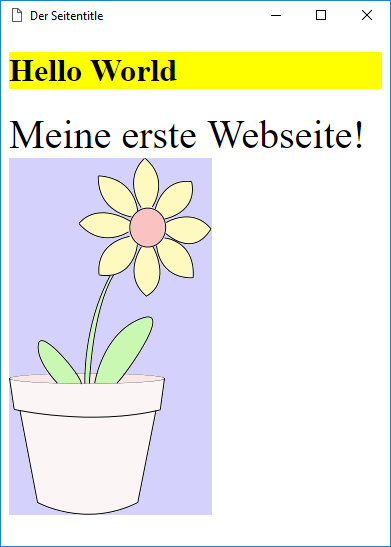
\includegraphics[width=.5\textwidth]{css.png}
		\caption{HTML erweitert mit CSS im Browser dargestellt}
		\label{img:css}
	\end{center}
\end{figure}

Die Zeilen 6-8 in \autoref{lst:css} heißen CSS-Anweisungen\index{CSS!CSS-Anweisungen}. Der linke Teil ist der Selektor\index{CSS!Selektor}\index{Selektor|see{CSS Selektor}} und gibt an, welche Elemente von der Regel betroffen sind. Der rechte Teil innerhalb der geschweiften Klammern ist die Deklaration. Diese besteht wiederum aus Paaren von Eigenschaften und Werten. Eigenschaft und Wert sind durch einen Doppelpunkt getrennt. Die Paare sind durch ein Semikolon getrennt. Mehrere CSS-Anweisungen ergeben zusammen ein Stylesheet\index{CSS!Stylesheet}\index{Sytlesheet|see{CSS Stylesheet}}.